\documentclass[tikz,border=10pt]{standalone}
\usetikzlibrary{angles}
\begin{document}
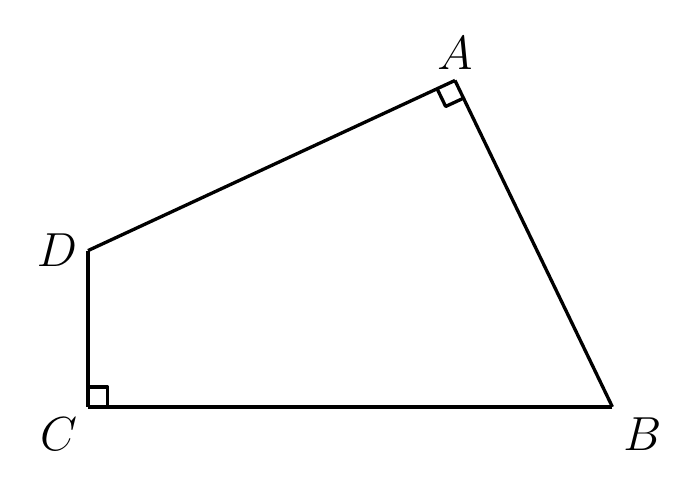
\begin{tikzpicture}[line width=1.2pt, line join=round]
\coordinate (A) at (1.336,2.087);
\coordinate (B) at (3.335,-2.058);
\coordinate (C) at (-3.325,-2.058);
\coordinate (D) at (-3.325,-0.074);




\draw (A) -- (B);
\draw (B) -- (C);
\draw (C) -- (D);
\draw (D) -- (A);


\pic [draw, angle radius=0.250cm] {right angle=B--C--D};
\pic [draw, angle radius=0.250cm] {right angle=B--A--D};


\node[above, font=\fontsize{17}{20.4}\selectfont] at (A) {$A$};
\node[below right, font=\fontsize{17}{20.4}\selectfont] at (B) {$B$};
\node[below left, font=\fontsize{17}{20.4}\selectfont] at (C) {$C$};
\node[left, font=\fontsize{17}{20.4}\selectfont] at (D) {$D$};
\end{tikzpicture}
\end{document}